% !Mode:: "TeX:UTF-8"

\documentclass[1pt,onecolumn,a4paper]{article}
% \documentclass[twocolumn,a4paper]{article}
% -----导言区-----
\usepackage{xeCJK}    %中文排版支持
% \usepackage[hyperref,UTF8]{ctex}   %处理交叉引用链接
\usepackage{hyperref}   %处理交叉引用链接
\usepackage{graphicx}   %插图支持
\usepackage{fontspec}   %字体处理

% \setCJKmainfont{STBaoliTC-Regular}
% \usepackage{syntonly}   %只编译不生成文档
% \syntaxonly

% -----定义区-----
% !Mode:: "TeX:UTF-8"

\graphicspath{{figures/}}   %图片路径定义

\setmainfont{TimesNewRomanPSMT}   %字体定义MAC OSX
\setsansfont{ArialMT}
\setmonofont{Courier}
\setCJKmainfont[BoldFont={STHeitiSC-Medium},ItalicFont={STKaitiSC-Regular}]{STSongti-SC-Regular}
% \setCJKsansfont{ }
% \setCJKmonofont{ }

% -----字号定义-----%
\newcommand{\chuhao}{\fontsize{42pt}{\baselineskip}\selectfont}     %初号
\newcommand{\xiaochuhao}{\fontsize{36pt}{\baselineskip}\selectfont} %小初号
\newcommand{\yihao}{\fontsize{28pt}{\baselineskip}\selectfont}      %一号
\newcommand{\erhao}{\fontsize{21pt}{\baselineskip}\selectfont}      %二号
\newcommand{\xiaoerhao}{\fontsize{18pt}{\baselineskip}\selectfont}  %小二号
\newcommand{\sanhao}{\fontsize{15.75pt}{\baselineskip}\selectfont}  %三号
\newcommand{\sihao}{\fontsize{14pt}{\baselineskip}\selectfont}       %四号
\newcommand{\xiaosihao}{\fontsize{12pt}{\baselineskip}\selectfont}  %小四号
\newcommand{\wuhao}{\fontsize{10.5pt}{\baselineskip}\selectfont}    %五号
\newcommand{\xiaowuhao}{\fontsize{9pt}{\baselineskip}\selectfont}   %小五号
\newcommand{\liuhao}{\fontsize{7.875pt}{\baselineskip}\selectfont}  %六号
\newcommand{\qihao}{\fontsize{5.25pt}{\baselineskip}\selectfont}    %七号

% -----命令定义-----%
\newcommand{\upcite}[1]{\textsuperscript{\textsuperscript{\cite{#1}}}}    %定义上角标引用
\renewcommand{\refname}{参考文献}   %中文名称



\title{测试中文文档\thanks{aab}}    %标题信息
\author{yanghaa}   %作者信息
\date{}

\begin{document}
  \maketitle
  % \tableofcontents

  % !Mode:: "TeX:UTF-8"

% \chapter{测试}
\section{测试2}
\subsection{subsection name子}
\subsubsection{afdf啊啊啊}
% \part{111}
\paragraph{一段文字}
\subparagraph{子段落文字}

一段文字\footnote{测试脚注},测试引用图片\upcite{RN3},如图~\ref{fig:1}
% dsad\\
%   {\chuhao 爱迪生多撒多c} \\
%   {\xiaochuhao 爱迪生多撒多xc}\\
%   {\yihao 爱迪生多撒多1}\\
%   {\erhao 爱迪生多撒多2}\\
%   {\sanhao 爱迪生多撒多3}\\
%   {\sihao 爱迪生多撒多4}\\
%   {爱迪生多撒多MR}\\
%   {\xiaosihao 爱迪生多撒多x4}\\
%   {\wuhao 爱迪生多撒多5}\\
%   {\liuhao 爱迪生多撒多6}\\
%   {\qihao 爱迪生多撒多7}
%

%
% 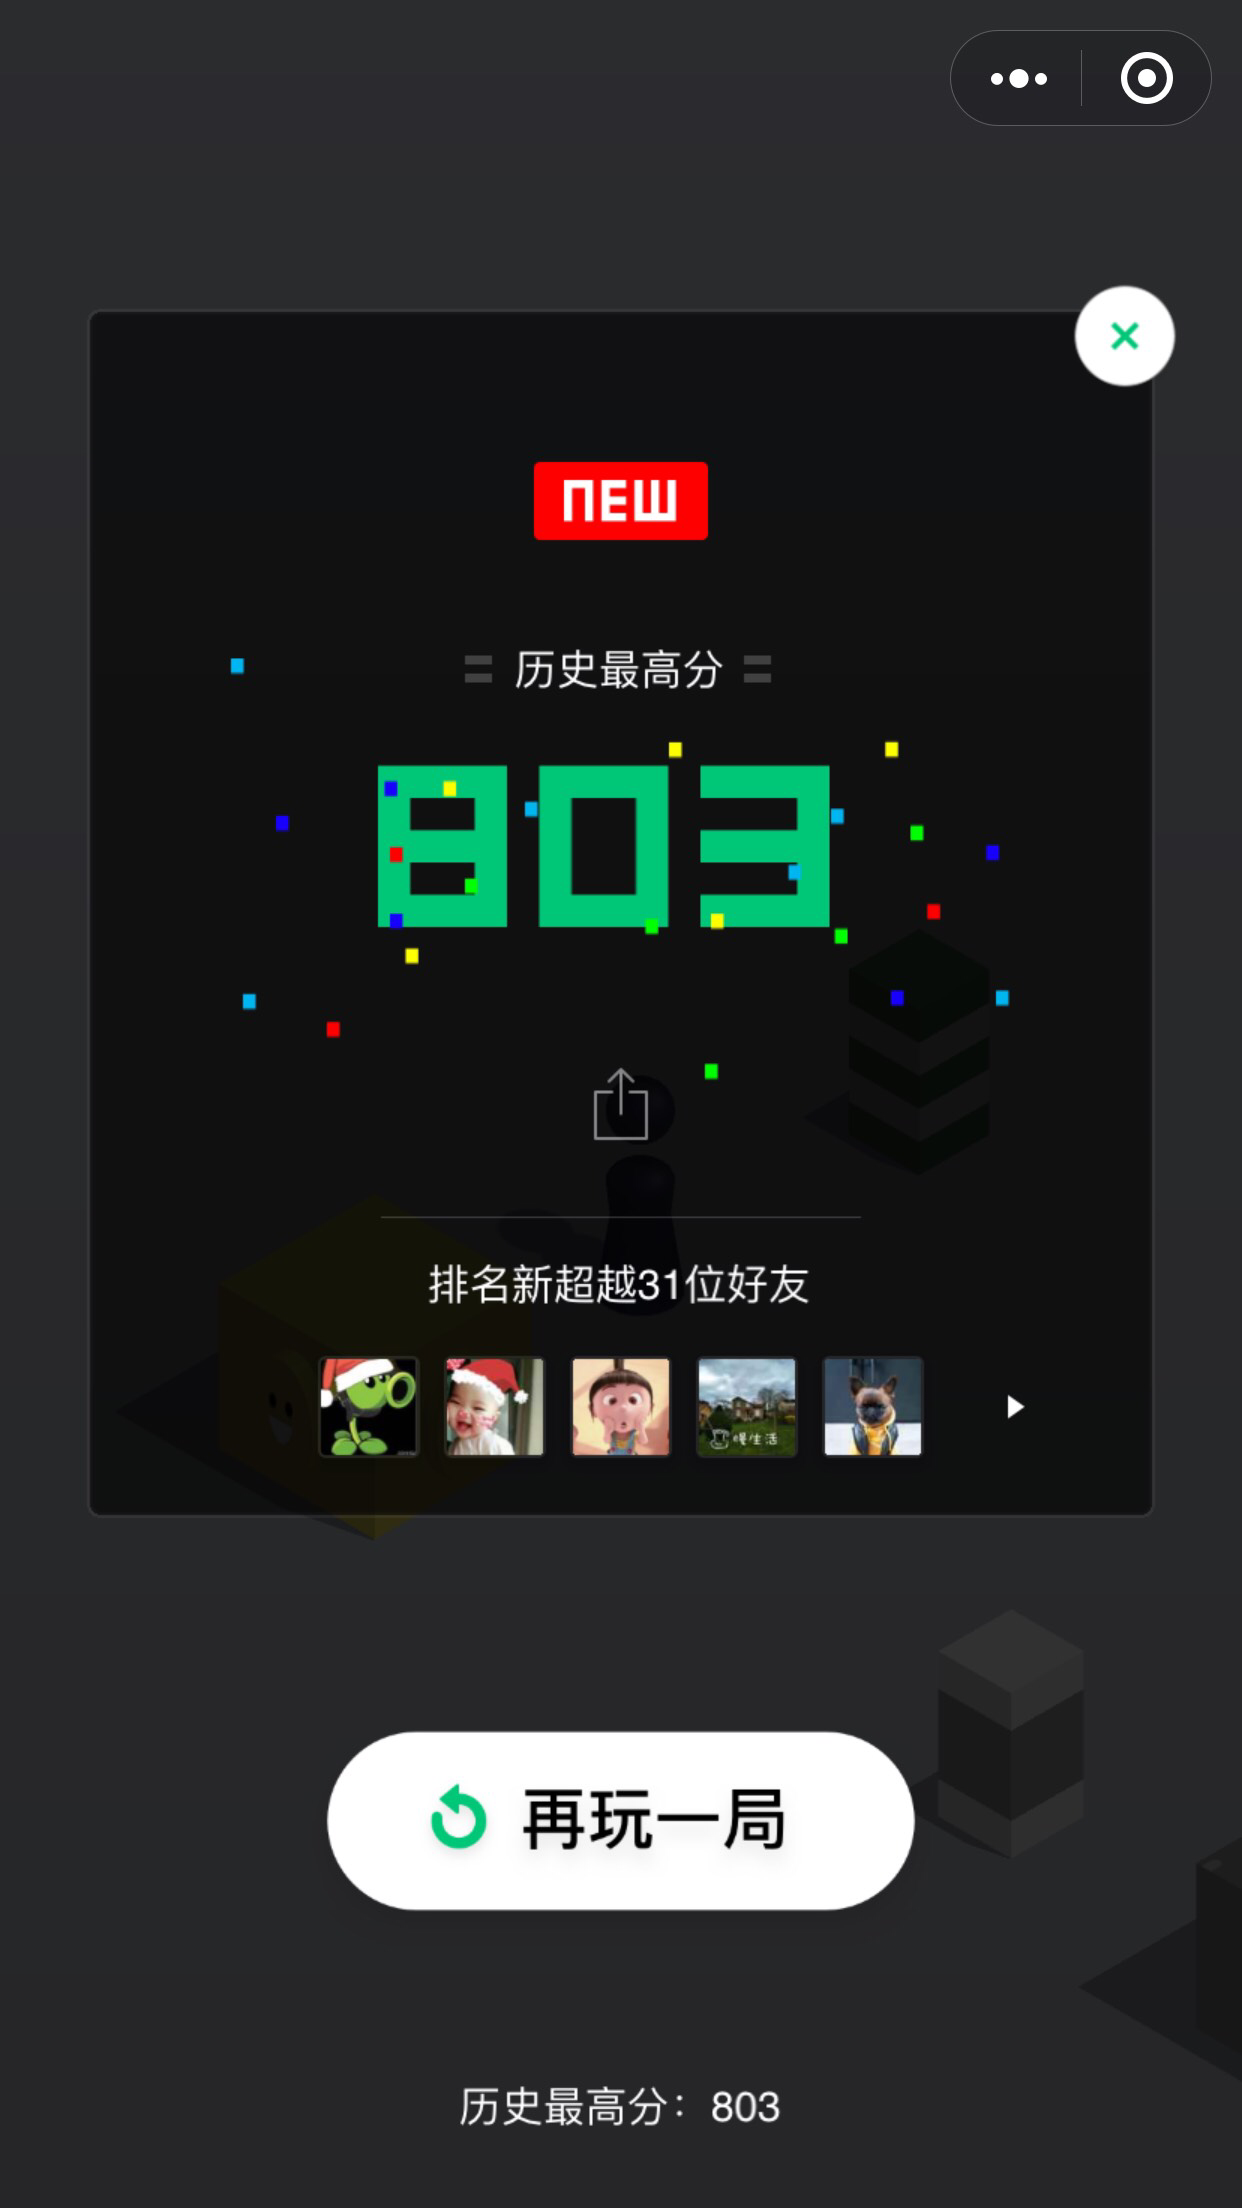
\includegraphics[height=2cm]{1.png}
%
\begin{figure}[t]
  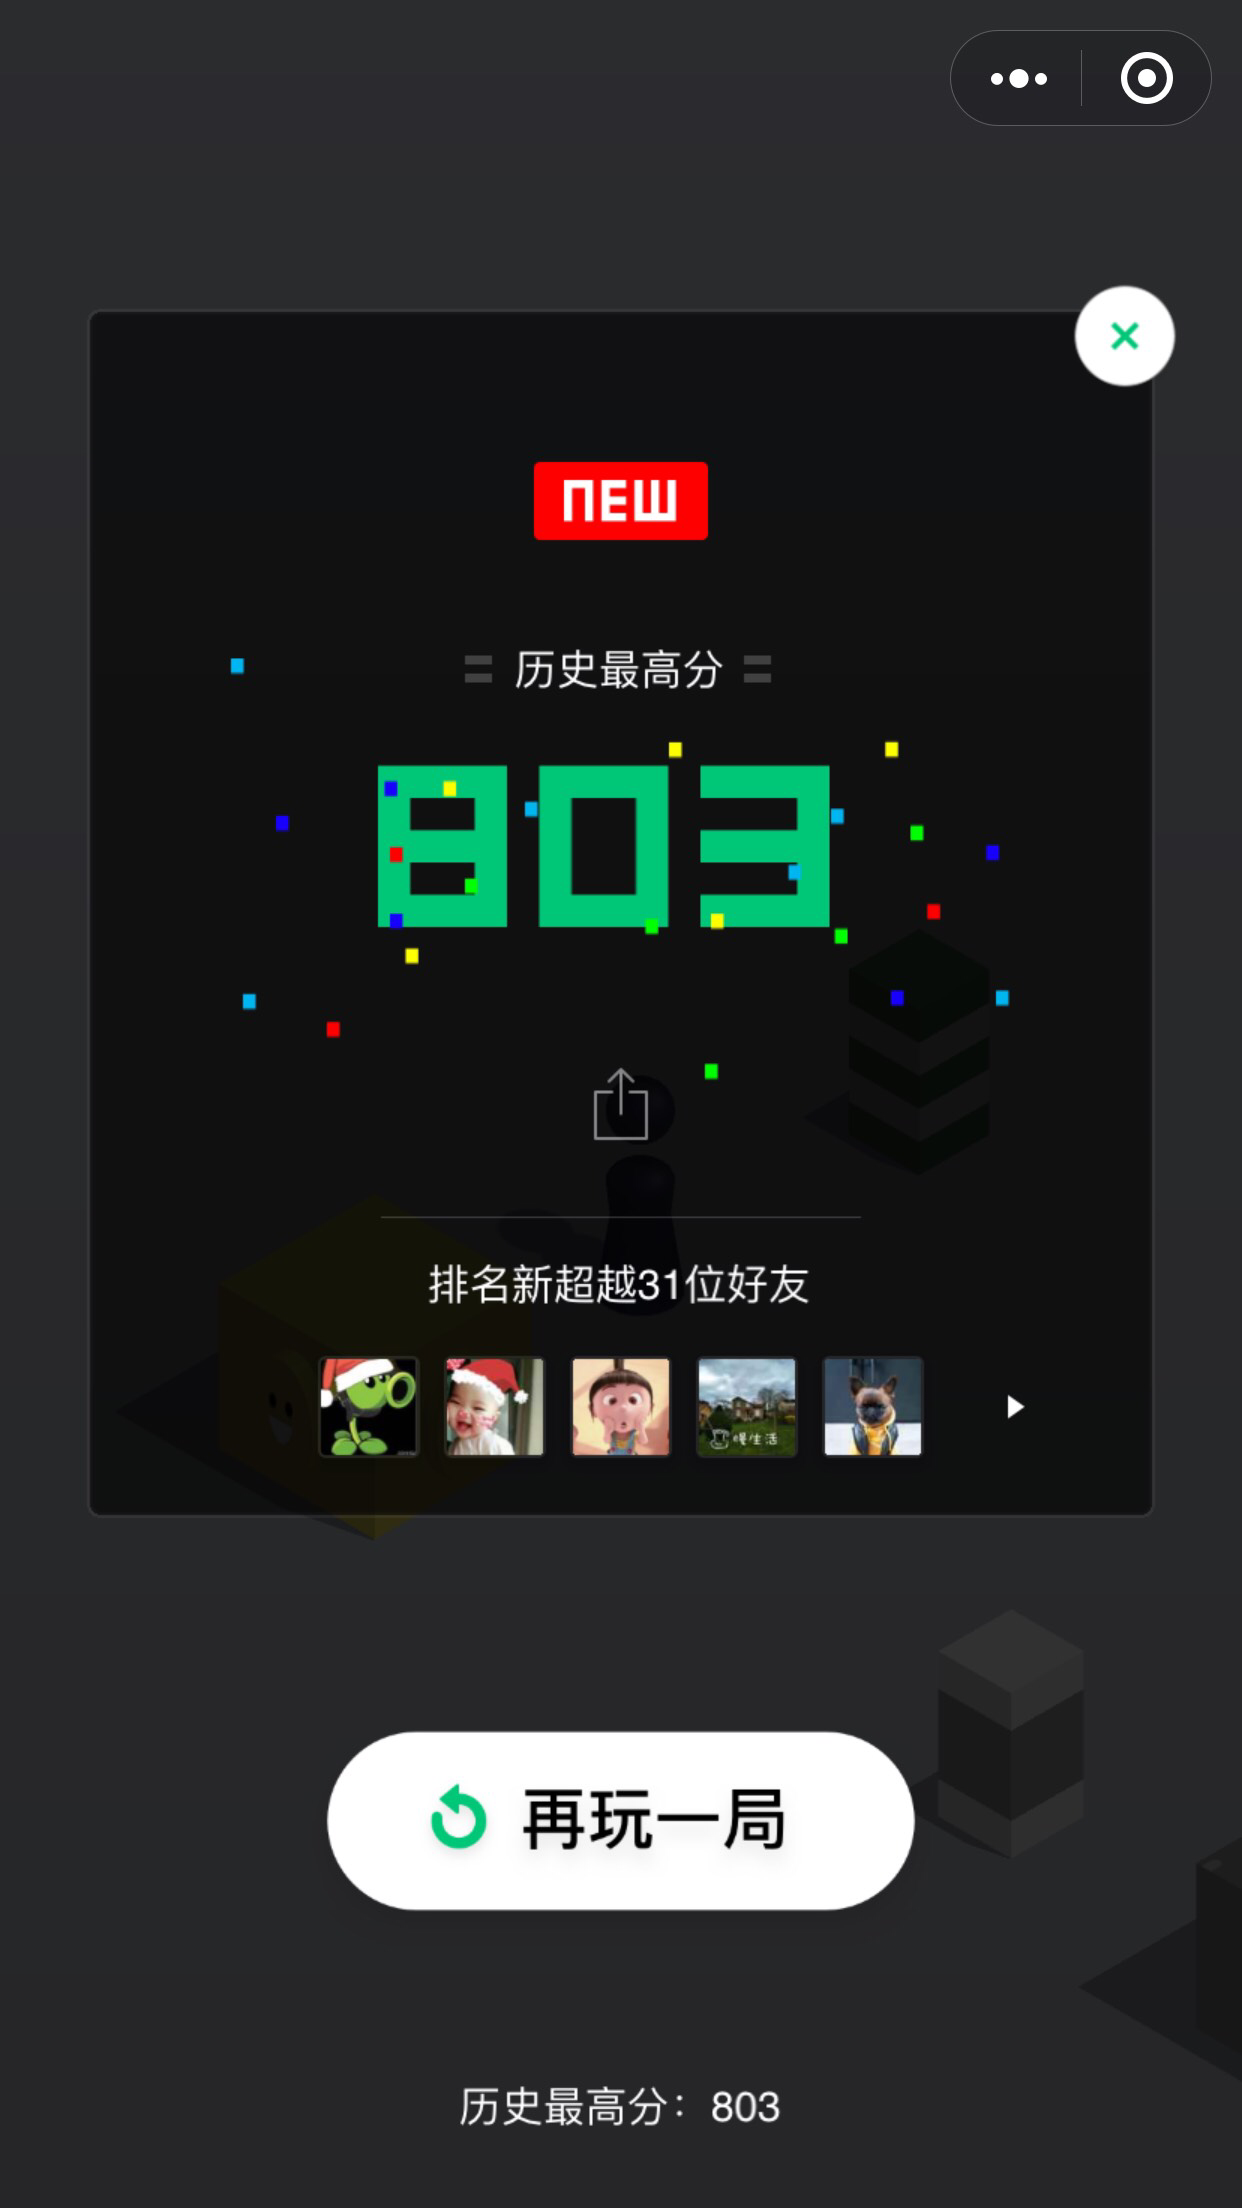
\includegraphics[height = 1 cm]{1.png}
  \caption{这是一张图}
  \label{fig:1}
\end{figure}

  \bibliographystyle{ieeetr}
  \bibliography{myref.bib}

  % !Mode:: "TeX:UTF-8"

\appendix

\section{附录1}
\section{附录2}
\section{附录3}






\end{document}
